\documentclass{beamer}
\mode<beamer>{%
\usetheme[hideothersubsections,
right,width=22mm]{Goettingen}
}
\usepackage[spanish]{babel} %Definir idioma español
\usepackage[utf8]{inputenc} %Codificacion utf-8
\title{Calificación de películas}
\author{Emmanuel Peto Gutiérrez\\Rodrigo Fernando Velázquez Cruz}
\institute{IIMAS \\ UNAM}
\begin{document}

\begin{frame}<handout:0>
\titlepage
\end{frame}

\section{Introducción}

% 1
\begin{frame}
\frametitle{Descripción del problema}

Los usuarios de servicios de streaming tienen problemas para seleccionar películas que le agraden y requieren una recomendación basado en lo que les ha gustado y lo que no les ha gustado.

\end{frame}

% 2
\begin{frame}
\frametitle{Objetivo}

Diseñar un sistema que filtre información sobre las películas y sobre los datos de los usuarios que han calificado las películas. También, mostrar estadísticas sobre los resultados filtrados.

\end{frame}

\section{Manager-Workers}

% 3
\begin{frame}
\frametitle{El patrón Manager-Workers}

Se utilizó el patrón de diseño en paralelo \textit{Manager-Workers}.

A continuación se explicarán los pasos realizados por el programa.

\end{frame}

% 4
\begin{frame}

\textbf{Paso 1}

Se calcula el número de hilos y se divide el archivo grande en $4p$ subarchivos, donde $p$ es el número de hilos disponibles en el CPU.

\begin{center}
\includegraphics[scale=0.6]{division}
\end{center}

\end{frame}

% 5
\begin{frame}

\textbf{Paso 2}

\begin{itemize}
\item Interpretar la información ingresada por el usuario, la cual es: selección de columnas y condición de filtrado para los registros.
\item El hilo principal le pasa al manager la información interpretada y el número de hilos.
\item El manager lanza $4p$ hilos y le pasa la consluta interpretada a cada uno.
\end{itemize}

\begin{center}
\includegraphics[scale=0.5]{lanzar}
\end{center}

\end{frame}

% 6
\begin{frame}

\textbf{Paso 3}

Una vez que el \textit{worker} conoce la consulta, aplica el filtrado y la selección sobre su subarchivo. Después, escribe sobre un archivo compartido, de manera sincronizada.

\begin{center}
\includegraphics[scale=0.6]{filtrado}
\end{center}

\end{frame}

% 7
\begin{frame}

\textbf{Paso 4}

Cuando ya se filtraron los subarchivos y se guardaron en el archivo compartido, se calculan estadísticas de forma secuencial como promedio, mediana, mínimo y máximo, y se muestran en gráficas de barras.

\begin{center}
\includegraphics[scale=0.6]{estadisticas}
\end{center}

\end{frame}

% 8
\section{Entrada y salida de datos}

\begin{frame}
\frametitle{Selección}

Primero, el usuario debe elegir los nombres de las columnas que desea seleccionar para el resultado. Estas se colocan en el campo de texto que está justo debajo de la etiqueta: \texttt{Indique las columnas a seleccionar.}

Las columnas que seleccione deben estar separadas por comas y las opciones son:

idRating, userId, movieId, rating, timestamp, title, year, genres, name, lastname, age, imdb, themoviedb.

\pause

Ejemplo, se pueden seleccionar las columnas: title, year, rating, genres.

\begin{center}
\includegraphics[scale=0.5]{seleccion}
\end{center}

\end{frame}

% 9
\begin{frame}
\frametitle{Condición}

Luego, se deben elegir las condiciones de filtrado y se deben escribir en forma normal disyuntiva.

Por ejemplo, se pueden filtrar los registros de ratings para todas las películas que hayan sido calificadas por personas de entre 20 y 30 años, para cualquier película que haya salido después del 2000, tal que su género sea Thriller u Horror con la siguiente expresión:

\pause

(age $>=$ 20 AND age $<=$ 30 AND year $>$ 2000 AND genres = Thriller) OR (age $>=$ 20 AND age $<=$ 30 AND year $>$ 2000 AND genres = Horror)

\begin{center}
\includegraphics[scale=0.3]{condicion}
\end{center}

\end{frame}

% 10
\begin{frame}
\frametitle{Resultados}

Los resultados se presentan en gráficas de barras y los datos que se observan son los de ratings: media, mediana, mínimo y máximo.

\begin{center}
\includegraphics[scale=0.3]{barras}
\end{center}

\end{frame}

\end{document}

